\chapter{Background}
In this chapter we establish the background for our work. We start by introducing the different entity matching approaches. Then we discuss the issues with the graph-based entity matching. We also introduce the cloud-based programming models. Finally we give an overview of the different clustering, blocking and partitioning methods that are used for entity matching.

\section{Entity Matching}
The groundwork of entity matching problem was first formalized by Fellegi and Sunter \cite{FESU69}. They give the problem a probabilistic foundation as posing the entity matching problem as classification problem \cite{RDGa11}. Since then a lot of approaches proposed to solve the problem of entity matching. 

\subsection{Attribute Based Entity Matching}
Traditional entity matching approaches are focused on pair-wise attribute similarities\cite{RDGa11}, i.e the similarity of the attribute values of the pair to match. Elmagarmid et al. \cite{EIVe07} give an overview of the similarity functions used.\\     
%Entity Matching problem can be described and solved as a supervised machine learning problem by using classification methods of data mining. \cite{FESU69} describe using Bayes method, \cite{McLe95} describe using decision trees and \cite{BiMo03} describe using SVM methods. Unsupervised machine learning methods can also be used, \cite{BhGe06} describe using Latent Dirichlet Allocation model. Koepcke and Rahm\cite{KoRa10} compare several machine learning based systems systems (See table  ~\ref{table:EmFrameworks}).  
Shortcoming of this approach is that it cannot perform disambiguation, that is when having two references with the same name, they cannot be identified as separate entities when they belong to different entities\cite{RDGa11}.

\subsection{Relational Entity Matching}
Alternative approaches to the probabilistic approaches are the relational approaches. Relational approaches of entity matching take structural similarity into account by looking at the attributes of related references, and incorporates them into attribute similarity score \cite{BhGe04}. Relational approach avoid the complexity of the probabilistic approach by avoiding a formal probabilistic model, these approaches can handle complex relationships between different entities more easily and significantly faster as well \cite{BhGe04}.

\subsection{Collective Entity Matching}
In traditional entity matching approaches, matching decisions are made independently, that is the decisions of matching a pair or a group of records are made independently from all other groups or records in the data set(s) that are matched or deduplicated. These approaches therefore make local decisions without taking the characteristics of all records in the data sets into account.

Bhattacharya and Geetor\cite{BhGe07} introduced collective entity matching approach, which determine entities for co-occurring references jointly, rather than independently by using both attribute and relational information for determining the underlying domain entities\cite{Chri12}. The basic idea of collective entity matching approach is to calculate the similarities of all connections in the relationship graph that are ambiguous using information from the known relationships. Since different types of entities are available, the known relationship between one type of entities can help to disambiguate of other types of entities. 

In collective entity matching approach, matching decisions are aimed to be made in an overall collective fashion over all the records pairs or groups of the datasets to be matched. This approach works best when having different type of entities with certain relationships between them. These relations can be represented by a relationship graph. 

Several techniques are proposed to solve the entity matching problem in collective fashion. These techniques differ in how the relationship graph is generated from the underlying datasets, and how the iterative update of the graph attributes is conducted. Collective entity matching techniques employs either iterative or hierarchical clustering, or graph-based approaches.

The collective entity matching problem can be solved in an iterative fashion. It is based on the idea that determining two references refer to the same entity may in turn allow us to make additional inferences about their related references. Using the relational evidence for collective entity matching has the potential benefit of producing more accurate matching results as well as solving both the identification and disambiguation problem at the same time. However, the potential benefit comes at cost of additional algorithmic complexity due to the propagation of the dependence between different matching decisions which results in having higher computation complexity and thus reduced scalability to large datasets.

Kalashnikov and Mehrotra \cite{KaMe06} used a graph-based approach by building a relationship graph between different kind of entities that have different relations (see figure \ref{fig:graph_exm}). the entity matching decisions are conducted in an iterative approach where the unknown weights are updated based on the number of connections in the path that needs to be covered to get from one end of the connection to the other. 

\begin{figure}[]
\centering
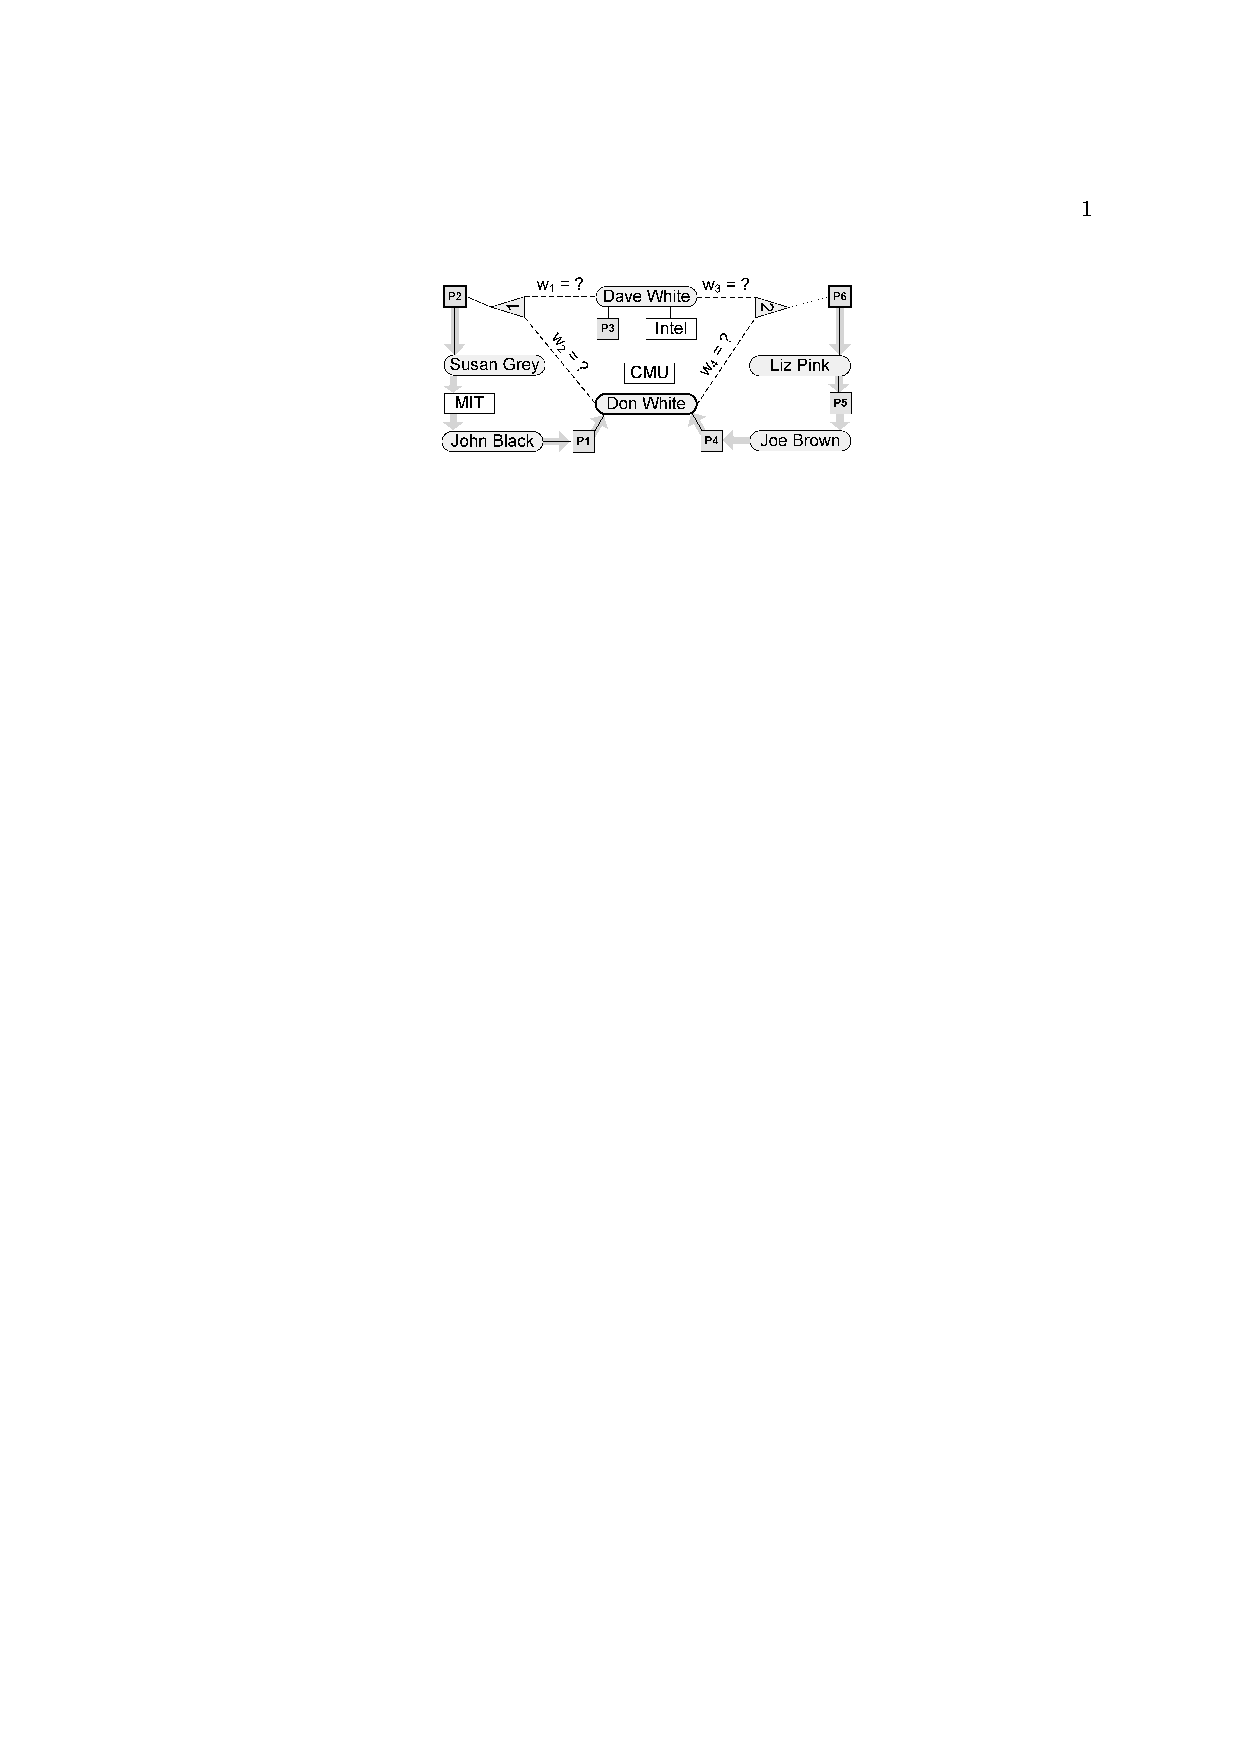
\includegraphics[page=1,trim = 35mm 218mm 0mm 45mm, clip] {figures/chapter3/fig4_cliping}
\caption{Graph for the publications example(\cite{KaMe06})}
\label{fig:graph_exm}
\end{figure}  


Another graph-based approach is proposed by Dong et al. \cite{DHMa05}, by constructing a dependency graph rather than a relationship graph. A node in the graph represents the similarity between a pair of entities of the same type, a connection between nodes occurs when this similarity depends upon the similarity of another pair of entities. %In this approach the collective entity matching is conducted in iterative fashion by initially marking all nodes as active. An active node is then selected, if similarity in that node is above certain similarity threshold it will be marked as merged, otherwise it will be marked as inactive. All neighborhood of this node that have similarity below 1.0 are marked as active. the set of Active nodes are maintained through a queue, and in each iteration the similarity of the node at the top of the queue is recalculated. The process continues until no active node is left in the queue and all nodes are wither marked as merges or inactive \cite{Chri12}.

Bhattacharya and Geetor \cite{BhGe07} proposed hierarchical clustering approach for collective entity matching. The collective entity matching is conducted using a priority queue. %The queue contains tuples each consists of two cluster identifiers and the similarity between the two clusters. the tuples are sorted according to the highest similarity. An iterative algorithm merges clusters and update the similarities between newly formed clusters as long as there are pairs of clusters in the queue that have a certain minimum similarity. When two nodes or clusters are merged, the similarities between the newly formed cluster and all its neighbors in the relational graph are update, and the similarities between older clusters and the new cluster are added into the priority queue. The algorithm stops when no more clusters can be merged when the similarity between them is below the minimum threshold\cite{Chri12}.
     
Collective entity matching approaches may produce more accurate results over using only attribute similarity measures but at the cost of additional algorithmic complexity resulting from propagating the dependence between different resolution decisions \cite{BhGe07}.

\section{Graph-Based Entity Matching}
Graphs have natural support for representing the relationships between references. When using graphs structure to represent the references and the relationships among them, the graph has nodes for each entity reference, in case of multi-type entity references, multiple node types is used. Graph edges represent relationships between references, when having different types of relations, edges with different types can be used to represent the different types of relations that exist. Sometimes relation involves more than two references like the co-author relation, in such situation the edge is not suitable to represent relation among more than two references, instead hyper-edge is used to span all the authors who co-authorize a paper\cite{BhGe06b}.
  
\subsection{Issues with Graph-based Entity Matching}
There are several interesting issues we encounter when using graphs for solving the entity matching problem. In this section we introduce some of these issues\cite{BhGe06b}.  
\subsubsection{Multi-Type Entity Matching}
In the traditional entity matching approaches, references of single-type entities are considered for the matching task. In graph-based entity matching, multiple types of entities can be solved simultaneously. 
\subsubsection{Collective Entity Matching}
When the entities are related, matching decisions can be made collectively since the matching decisions depend on each other. For example in the citation domain, the relevant entities are authors, papers and venues and the relevant relationships between them are write and published in,  that is an author write papers, which get published in venues. An author is a co-author of another author if they write the same paper. Having this situation, one matching decision will lead to another.
\subsubsection{Positive and Negative Relational Evidence}
Other relations may be useful to be used as relational evidence. These relations might be positive like the cited by relation when paper is cited by another paper, co-cited relation when two papers are cited by the same paper entity. If two similar paper references are co-sited by the same paper entity, then this gives us additional evidence that they are the same. Relations may also lead to negative matching evidence like the case when two paper references are cited by the same paper entity, then it is unlikely that these two papers are duplicates.

\subsection{Graph-based Similarity}
The task of entity matching may be viewed as a graph-based clustering problem where the goal is to cluster references so that references that have identical entity labels are in the same cluster. In this section, we address the graph-based similarity measures between entity clusters based on considering the entities that they are related to via the observed edges\cite{BhGe06b}. 

\subsubsection{Edge Detail Similarity}
% To add here, section 5.2.1 of entity resolution in graphs
In graph-based clustering, we have each entity cluster associated with a set of edges to which the references contained in it belong. Recalling that each reference $r$ is associated with a hyper-edge $r.H$, then the edge set $c.H$ for an entity cluster c may be defined as $c.H=\{r.H=h, r\in c\}$     . We define a similarity measure for a pair of edges that can be used to measure the relational similarity between two clusters. What is relevant for the similarity in  relational clustering are the clusters labels of the references in each edge, so for each edge, we consider the multi-set of entity labels, one for each reference associate with it. We employ the Jaccard similarity measure over these multi-set of entity labels. Let $label(h_i)$ be the set of entity labels for an adge $h$. Then for a pair of edges $h_i$ and $h_j$, we define their similarity as:  

%\begin{align*}
$$sim(h_i,h_j)=\frac{|label(h_i)\cap label(h_j)|}{|label(h_i)\cup label(h_j)|}$$
%\end{align*}

Now, given this similarity measure, we can calculate the graph-based similarity between two entity clusters using an aggregation operator like $max$ as follows:
%\begin{align*}
$$sim_{graph}(c_i,c_j)=max_{(h_i,h_j)}\{sim(h_i,h_j)\}, h_i \in c_i.H,h_j \in c_j.H$$
%\end{align*}

Since it explicitly considers every edge associated with each entity cluster, we call this \textit{edge detail similarity}. The computation of the  \textit{edge detail similarity} of two clusters is quadratic in the average number of edges associated with each cluster.
 
\subsubsection{Neighborhood Similarity}
% To add here, section 5.2.2 of entity resolution in graphs
If entity clusters have the same edge structures, that is the same neighbor cluster to which they have edges, this gives sufficient graph-based evidence that these entities should be matched.
Recall that $label(l)$ is defined as the multi-set of entity labels for an edge $h$ and for an entity cluster $c$, $c.H$ is the set of edges associated with it. Then the neighborhood multi-set $c.N$ for $c$ can be formally defined as follows:

%\begin{align*}
$$c.N=\bigcup_m {label(h_i)},h_i \in c.H$$
%\end{align*}
   
where $\bigcup_m$ is the multi-set union operator. Intuitively, we are looking at how many times $c$ has participated in the same edge with another entity cluster,excluding $c$ it self. Next, To calculate the graph-based similarity measure between two entity clusters, we calculate the Jaccard similarity between their neighborhood multi-sets.

%\begin{align*}
$$sim_{graph}(c_i,c_j)=\frac{|C_i.N)\cap C_j.N)|}{C_i.N)\cup C_j.N)|}$$
%\end{align*}

We call this \textit{neighborhood similarity} between the two entity clusters. The computation and update of neighborhood similarity is significantly cheaper, in terms of computation, compared to edge detail similarity.

\section {Cloud-based Programming Models}
In this section we introduce the programming models suitable for the cloud-based platforms. We introduce MapReduce and Pregel programming models.
\subsection{MapReduce Programming Model}
MapReduce\cite{DeGh08} is a distributed programming model that is dedicated for complex and distributed computations. It enables the parallel programming on hundreds or even thousands of shared nothing commodity PCs clusters. This programming model hides the details of the parallelism complexities and provide simple programming model consists of two functions, Map and Reduce. In the Map function the programmer specifies the computation need to be carried out in parallel fashion by the underlying hardware, the map function process the input in the form of key/value pair (which is the basic data structure of MapReduce), the computation is carried out in distributed fashion and an intermediate results are generated in the form of key/value pairs. In the Reduce function, all the intermediate values associated with the same intermediate key are merged and the final result of the computation is produced. 
MapReduce divides the processing into two consecutive stages: the map and the reduce phase. The mechanism works as follows: the input starts as data stored in distributed system, the mapper is applied to every key value pair to generate an arbitrary number of intermediate key/value pairs and then the reducer is applied to all values associated with the same intermediate key to generate out key/value pairs, implicit between the map and reduce is distributed group by operation in intermediate keys (see figure \ref{fig:mapreduce}).

MapReduce has not been originally designed for graph-processing, However a set of good practices along with design patterns for graph processing have been developed. These good practices show how to express iterative algorithms in MapReduce, however they are helpless in overcoming the inefficiencies of MapReduce model in graphs processing\cite{KIK*12}. The reasons of the inefficiencies of MapReduce when processing graphs are the great network overhead since the graph structure must be transferred over the network of computational nodes from Mappers to Reducers so that they can serve as an input for the next iteration.  The stateless, two-phased computational nature of MapReduce does not allow vertices to reside on the same machine throughout the whole computation.  After every phase (map/reduce) the entire data must be written to a global memory in order to be consumed in the next phase. Since the distributed file system serves as the global memory in the cloud environment, the whole computation is very disk-intensive. Additionally, the map and reduce workers reside on different physical machines and for that reason, the data is constantly transferred over the network, which is the scarce resource in cloud environment\cite{KIK*12}.

\begin{figure}[H]
\centering
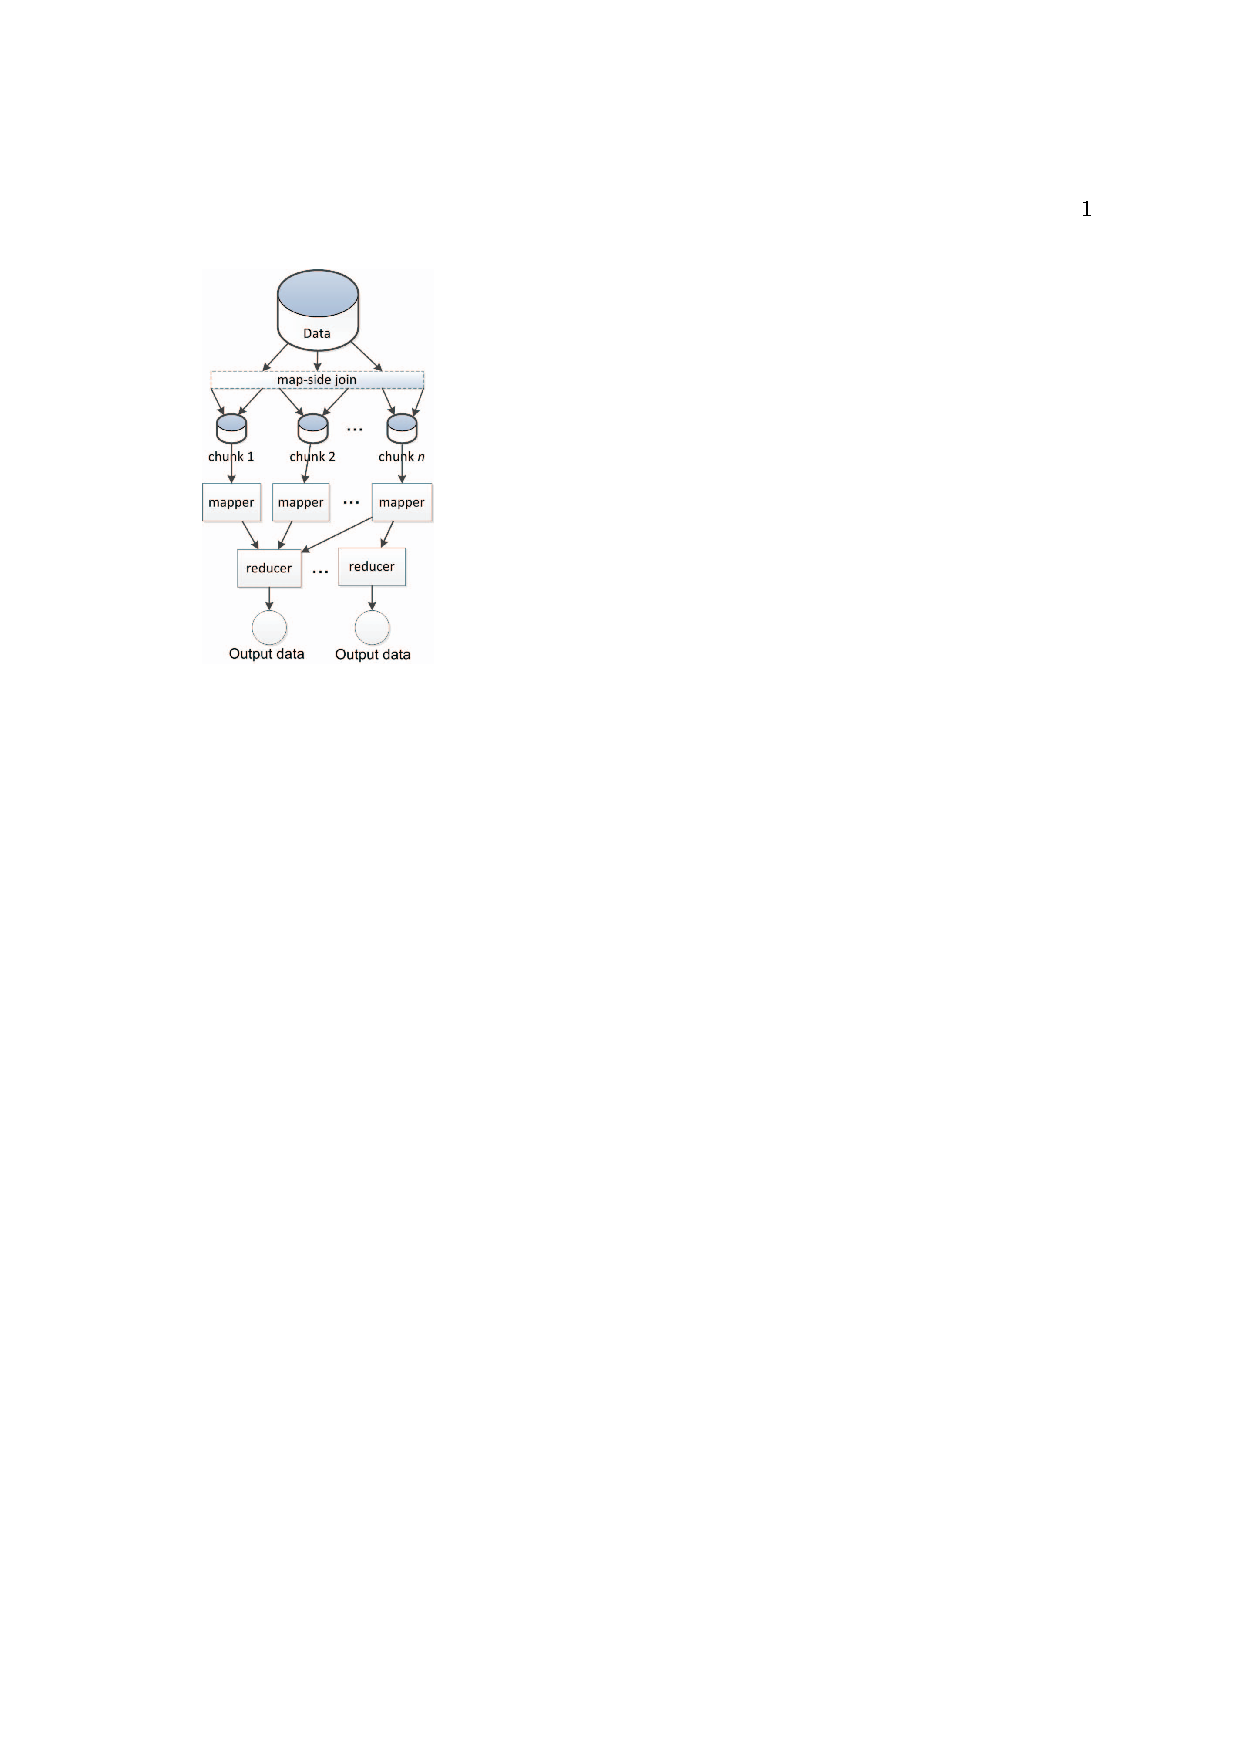
\includegraphics[page=1,trim = 30mm 185mm 135mm 45mm, clip]{figures/chapter3/fig5_cliping}  
\caption{Data flow in MapReduce programming model(\cite{KIK*12})}
\label{fig:mapreduce}
\end{figure}
\subsection{BSP Programming Model}

Having in mind the inefficiency of MapReduce for iterative graph processing, Google has created Pregel \cite{MAB*10} - a distributed, fault-tolerant system for graph processing, based on Bulk Synchronous Parallel (BSP) processing model \cite{Vali90}. 

The computation in the BSP model is organized as a sequence of supersteps. Each superstep consists of two phases, the computational phase followed by the communication phase. In the computational phase, local independent computations run in parallel by the processors. In the communication phase, processors communicate data in all-to-all fashion. Between two supersteps there is a synchronization barrier that guarantees the simultaneous start of all the processors for the next step. The global synchronizations at the end of each superstep have significant advantages for large scale distributed systems since it ensures avoiding the overlapping of communication and computation phases and provide a straightforward way to store consistent partial states in checkpoints. In BSP, the computation consists of a series of supersteps. In every superstep, a user defined function is executed in parallel on every item from the dataset acting as an agent. Pregel is vertex-centric: a single agent computation has a graph representation in BSP. It consists of a node identifiers, its current value and/or state, and a list of nodes outgoing edges. 
In Pregel , all processing is carried out on the machines local memory. Before the computation, all vertices are partitioned and loaded into local memories of machines and remain there throughout the entire computation. In every superstep, a vertex receives messages from other vertices and executes a user defined function compute(), which performs local processing and sends messages to some or all of its neighbors. Once a vertex finishes the local computation, it deactivates itself and waits for all other vertices to finish. The barrier of synchronization mechanism allows the next superstep to begin when all vertices complete processing in the current superstep. Then only the vertices that have received a message are activated\cite{KIK*12}((see figure \ref{fig:bsp}).

The BSP model has a stateful nature  that facilitates efficient graph computing since graph’s structure does not need to be send over the network. Only specific messages necessary for the algorithm execution are exchanged. There is no network overhead related to graph structure passing as in the MapReduce model. Moreover, storing the whole graph structure in local memory of workers allows in-memory computation such that there should be no need of disk write-reads between iterations. However, it this is possible only if the graph structure fits in memory of all workers. Otherwise, the spilling-to-disk techniques must be implemented\cite{KIK*12}.
\begin{figure}[H]
\centering
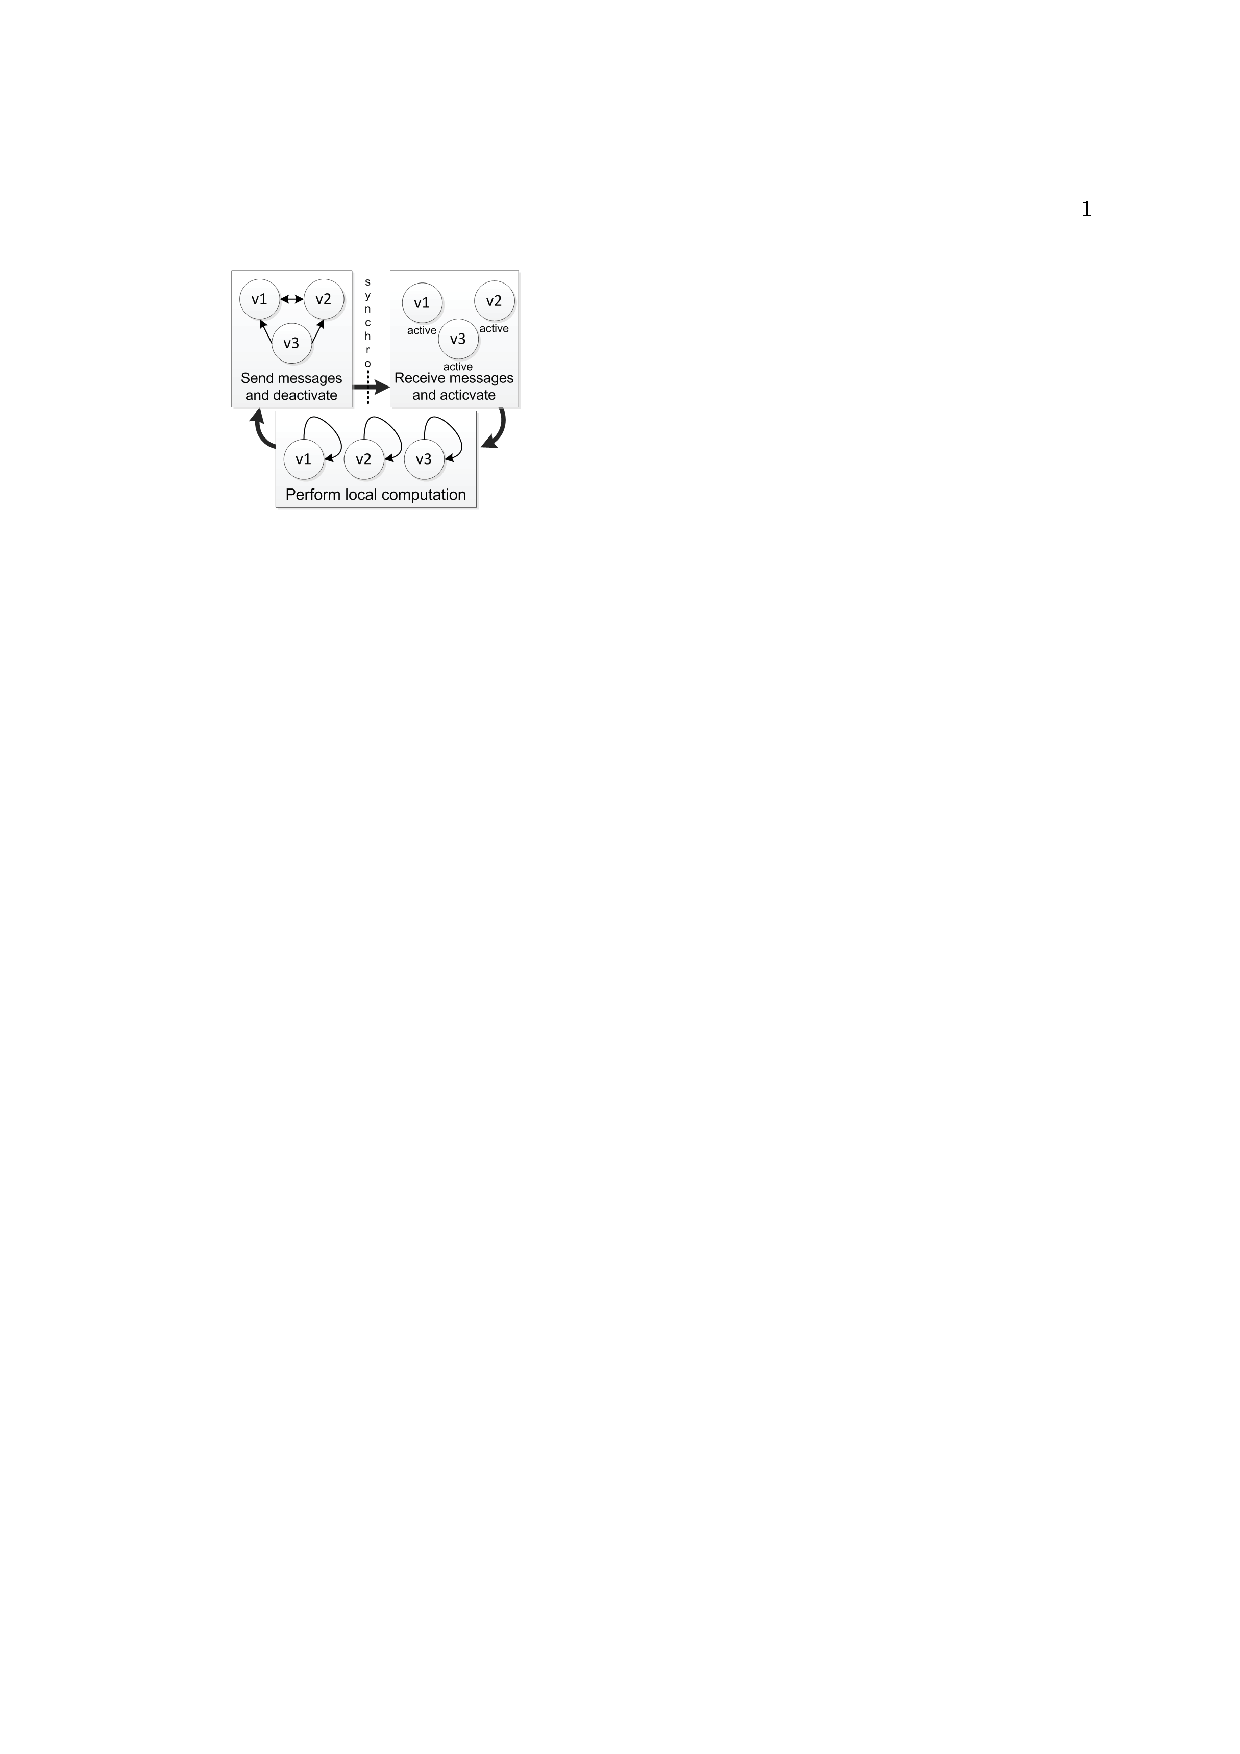
\includegraphics[page=1,trim = 35mm 210mm 120mm 45mm, clip]{figures/chapter3/fig6_cliping}  
\caption{Data flow in MapReduce programming model(\cite{KIK*12})}
\label{fig:bsp}
\end{figure}

\section{Clustering Approaches}
The task of entity matching may be viewed as a clustering problem where the goal is to cluster the references so that those that have identical entity labels are in the same cluster.The key to the success of a clustering algorithm is the similarity measure that is employed\cite{BhGe06b}. Different clustering methods were proposed for the entity matching problem, in this section we give an overview of these methods:

\subsection{Relational Clustering}
Bhattacharya and Getoor\cite{BhGe06b} Propose using greedy agglomerative clustering approach for the collective relational entity matching approach. At any stage of the clustering algorithm, each constructed entity cluster should correspond to one underlying entity and all references in that cluster should be to that entity. The greedy agglomerative clustering algorithm start by having each reference belong to separate cluster and at each step the pair of cluster that are most likely to refer to the same entity are merged.

\subsection{Component-based Clustering}
For graphs based clustering, component-based clustering can be used. Component-based clustering is based on the more general single-link hierarchical clustering method. The connected-components clustering method can be shown to be an instance of the single link method\cite{KMP*09}. Specifically, if d(n) is the distance of the two clusters to merge at step n of the single-link method, and G(n) is the graph that links all data points within distance of at most d(n), then the clusters after step n are the connected components of G(n)\cite{KMP*09}.

\subsection{Semi-clustering}
Semi-clustering, arises in social graphs. Social graphs are analogous to the graph of references with the relationships among those references. In social graphs, vertices typically represent people and edges represent the relationships between them. edges may have weights to represent the frequency of interactions or the strength of the relationship\cite{MAB*10}.

A semi-cluster in asocial graph is a group of people who interact frequently with each other and less frequently with others\cite{MAB*10}. Semi-cluster is distinguished from ordinary clustering approaches in that vertex may belong to more than one semi-cluster \cite{MAB*10}. This is similar to the canopies blocking technique where the vertex can belong to more than one canopy resulting in having overlapping canopies.

A semi-cluster $c$ is assigned a score as following\cite{MAB*10}:

%\begin{align*}
$$S_c=\frac{I_c-f_BB_c}{V_c(V_c-1)/2}$$
%\end{align*}  

where $I_c$ is the sum of the weights of all internal edges, $B_c$ is the sum of the weights of all boundary edges (i.e., edges connecting a vertex in the semi-cluster to one outside it), $V_c$ is the number of vertices in the semi-cluster, and $f_B$, the boundary edge score factor, is a user-specified parameter, usually between 0 and 1. The score is normalized, i.e., divided by the number of edges in a clique of size $V_c$, so that large clusters do not receive artificially high scores\cite{MAB*10}.

  
\subsection{Clustering Aggregation}
This clustering approach is particularly effective in cases when the data are defined over heterogeneous attributes that contain incomparable values. Using this approach allows us to apply the suitable clustering approach for each data set and then aggregate the individual clustering into a single clustering\cite{GMTs07}.
% Description of the clustering aggregation approach

\section{Blocking methods}

Blocking improve the efficiency of entity matching by avoiding the evaluation of the complete Cartesian product of entities. it reduces the search space for entity matching by using some kind of semantic partitioning by grouping similar entities within blocks and by restricting entity matching to entities from the same block \cite{KKH*10}. In this section we give an overview of two blocking methods that are relevant to our work.


\subsection{Canopies}
Canopies\cite{MNUn00} are overlapping subsets of high-dimensional data set that is divided efficiently by using a cheap, approximate distance measures. An element may appear under more than one canopy, and every element must appear in at least one canopy. Canopies are created with the intention that points not appearing in any common canopy are far enough apart that they could not possibly be in the same cluster. Since the distance measure used to create canopies is approximate, there may not be a guarantee of this property, but by allowing canopies to overlap with each other, by choosing a large enough distance threshold, and by understanding the properties of the approximate distance measure, we can have a guarantee in some cases.

\subsection{Semantic Blocking}
Semantic blocking is new family of blocking algorithms\cite{NMM*07}. It substitutes typical blocking methods by another type of block building method that is based on the relations between the entities rather than the values of attributes the entity has. The basic idea that the semantic blocking is based on the idea that references of entities are more likely to refer to the real-life entity if they are closely related in the context established by their relations with other entities in the data set.

\section{Partitioning Strategies}
For parallel entity matching, good partitioning of data is essential to have balanced distribution of the data among the machines. Different partitioning strategies exist. One of the strategies is size-based partitioning to evaluate the Cartesian product for entity matching. The other strategy is blocking-based partitioning to combine blocking with parallel matching \cite{KKH*10}. 

\subsection{Size-based Partitioning}
Size-based partitioning is the simplest approach and is applied for evaluating the complete Cartesian product of input entities. The goal is to split the input entities into equally-sized partitions so that each match task has to match two such partitions with each other. This approach is thus very simple and the equally sized partitions promise a good load balancing and scalability to many nodes.

\subsection{Blocking-based Partitioning}
Evaluating the Cartesian product does not scale and is thus only feasible for small-sized match problems. For larger match problems the use of blocking becomes necessary to reduce the scope for matching. Blocking entails a logical partitioning of the input entities such that all matching entities should be assigned to the same output partition, also called cluster or block. By restricting the match comparisons to the entities of the same block the match overhead can often drastically be reduced.
